\section{Packet transactions}
\begin{figure}
  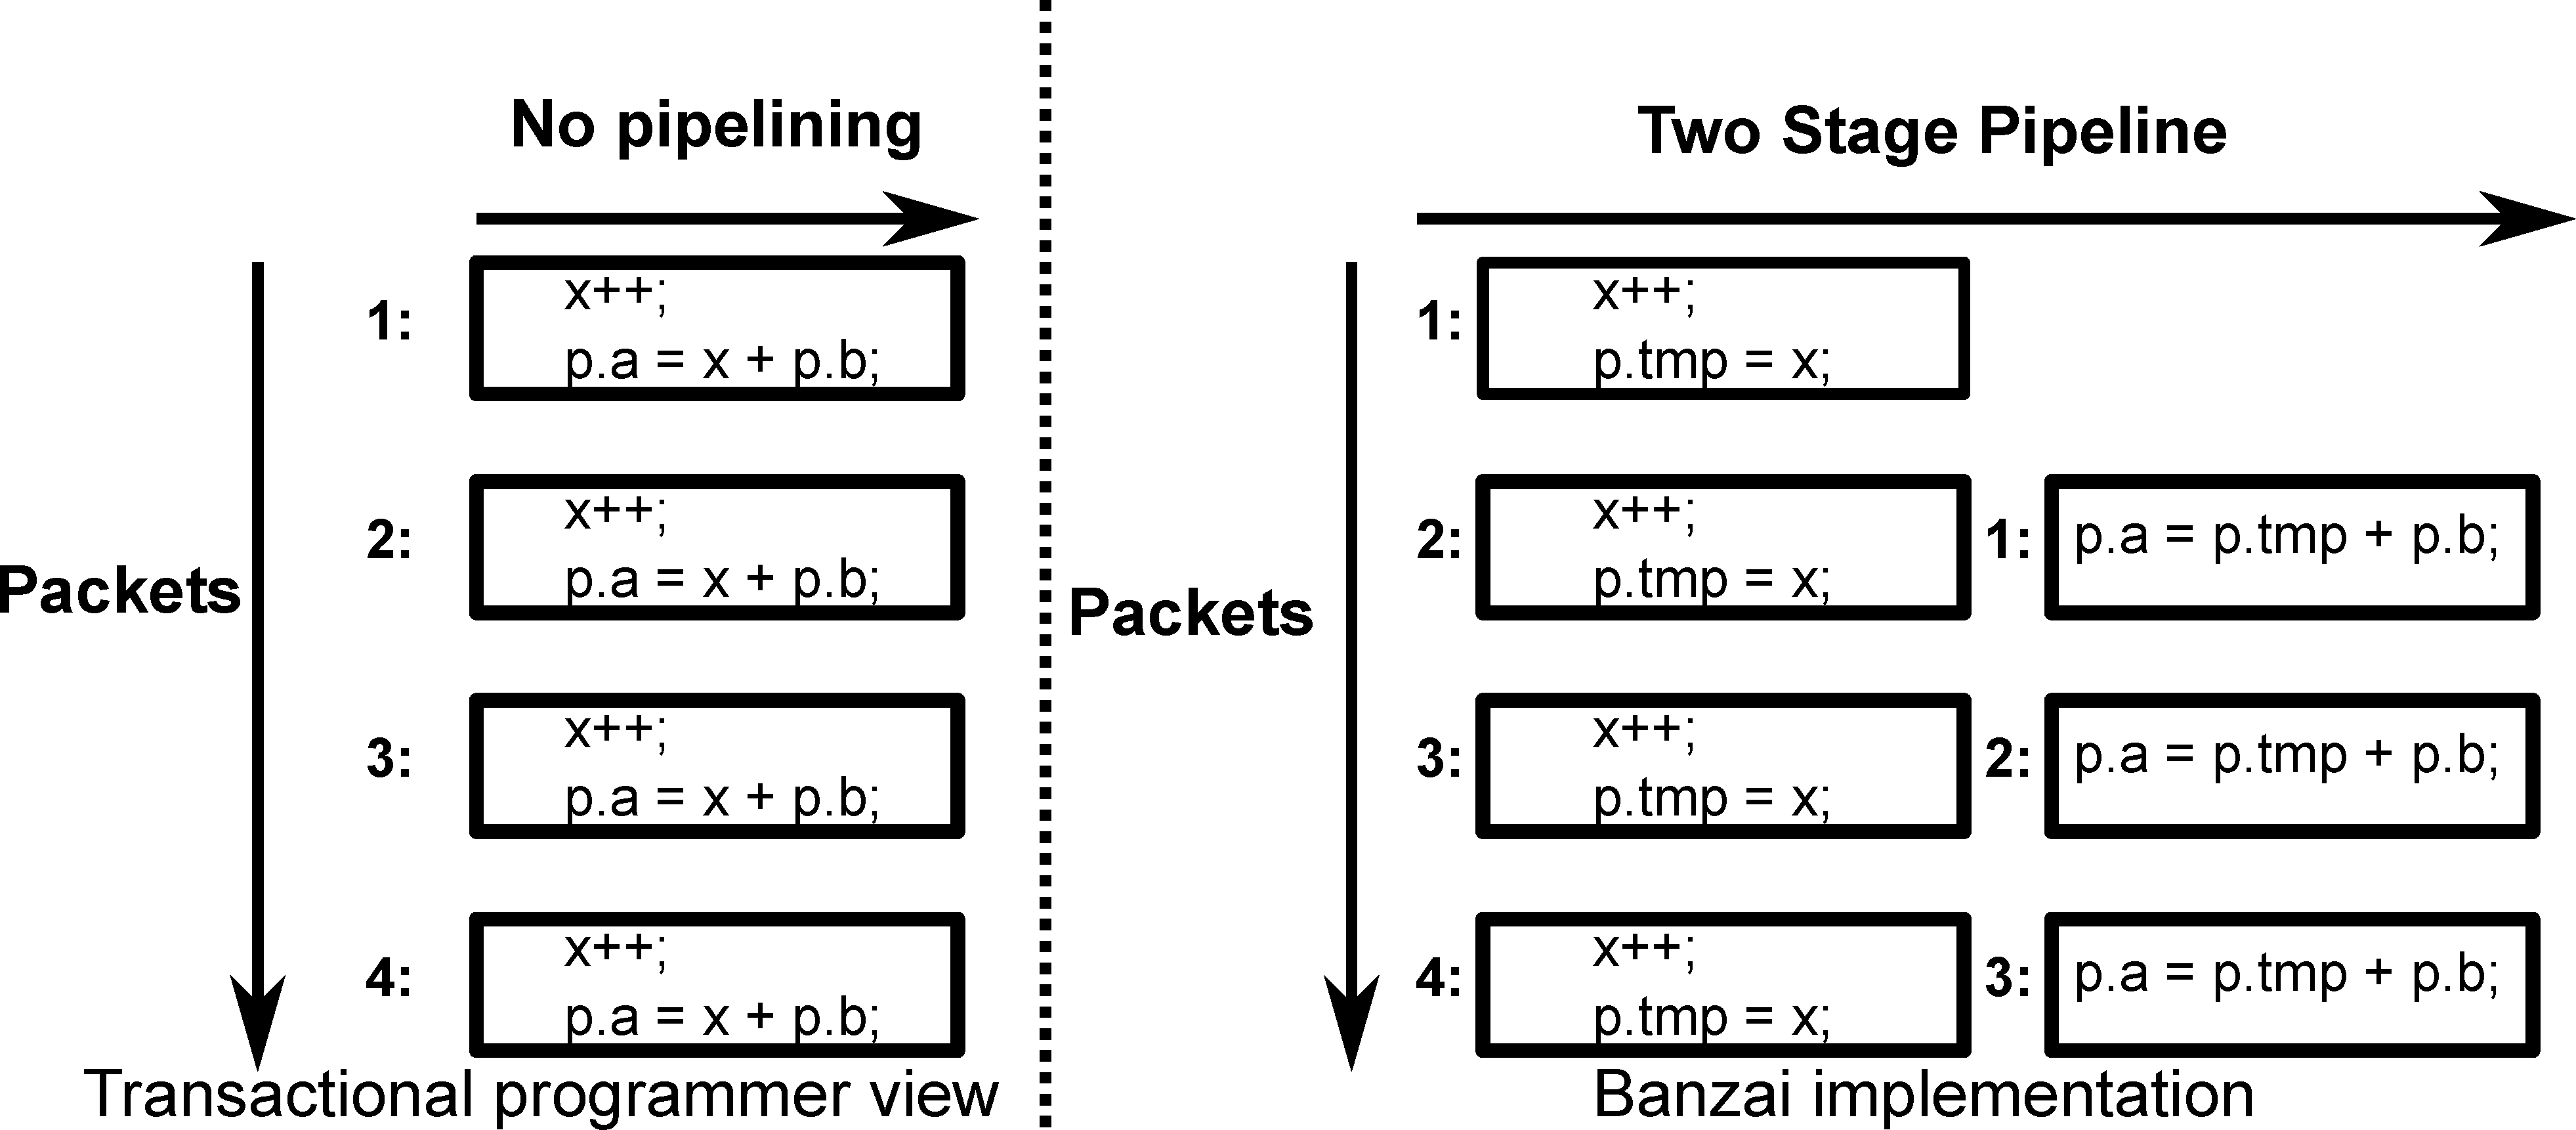
\includegraphics[width=\columnwidth]{spec_vs_impl.pdf}
  \caption{A packet transaction and its implementation}
  \label{fig:trans}
\end{figure}

Transactions are the strongest guarantee that a database system can provide in
that the effect of a transaction is either entirely visible or not with no
intermediate state being visible to the outside world.

We repurpose database transactions for data-plane programming by defining a
\textit{packet transaction}: a body of sequential code that executes from start
to finish on each packet and conceptually processes only one packet at a time.
For a programmer, the packet transaction represents what happens to every
packet without having to worry about other packets that are currently being
processed by the switch, how many pipeline stages it has, and how to
parallelize code. Conceptually, every packet is processed in isolation and to
completion using a sequential block of code before the next packet's processing
begins.

In practice though, switch hardware is heavily pipelined
(Figure~\ref{fig:switch}).  A compiler automatically translates the
programmer's transactional code block into a low-level pipelined implementation
on the switch hardware (Figure~\ref{fig:trans}).

% TODO: Add a flowlet switching example as a running example here.
As an illustration of programming in \pktlanguage, we consider how a programmer
would express a data-plane load-balancing algorithm such as flowlet
switching~\cite{flowlet} using domino. Flowlet switching is a load balancing
that harnesses the natural burstiness of TCP traffic to load balance set of
packets (called flowlets) separated by a large enough interval in time, called
the flowlet threshold. This flowlet threshold is chosen to ensure that packets
from flowlets taking different paths do not arrive out of order at a TCP
receiver, thereby causing it to reorder packets and degrade throughput.

Flowlet switching is conceptually simple to write down and can be expressed
as the C code block shown in:
\begin{figure}
\begin{small}
\begin{lstlisting}
#define NUM_FLOWLETS      8000
#define FLOWLET_THRESHOLD 5

struct Packet {
  int src_port;
  int dst_port;
  int src_addr;
  int dst_addr;
  int protocol;
  int new_hop;
  int arrival_time;
  int next_hop;
  int flow_hash;
};

int last_time [NUM_FLOWLETS] = {0};
int saved_hop [NUM_FLOWLETS] = {0};

void func(struct Packet pkt) {
  pkt.flow_hash = hash5(pkt.src_port, pkt.dst_port,
                        pkt.src_addr, pkt.dst_addr,
                        pkt.protocol);
  pkt.new_hop   = hash6(pkt.src_port, pkt.dst_port,
                        pkt.src_addr, pkt.dst_addr,
                        pkt.protocol, pkt.arrival_time);
  if (pkt.arrival_time - last_time[pkt.flow_hash \% NUM_FLOWLETS] >
      FLOWLET_THRESHOLD) {
    saved_hop[pkt.flow_hash \% NUM_FLOWLETS] = pkt.new_hop;
  }
  last_time[pkt.flow_hash \% NUM_FLOWLETS] = pkt.arrival_time;
  pkt.next_hop = saved_hop[pkt.flow_hash \% NUM_FLOWLETS];
}
\end{lstlisting}
\end{small}
\label{fig:flowlet}
\caption{Flowlet switching in \pktlanguage}
\end{figure}

% Mention language features here.

% TODO: Do we mention programmable parsers anywhere?
Here, the global arrays \texttt{last\_time} and \texttt{saved\_hop} represent
the last time a packet was received from a given 5-tuple and the saved value of
the next hop for that 5-tuple.\footnote{Hash function collisions can occur,
  leading to two flows sharing last\_time and saved\_hop values. As we explain
later in \S\ref{s:banzai}, this is unavoidable given the constraints on modern
switch architectures.}. The next\_hop packet field specifies the next hop
chosen for the packet, which can either be the saved value of next hop or a
newly computed value.

When compiled to the \absmachine abstract machine, the \pktlanguage compiler
converts the above code into the pipelined form shown in
Figure~\ref{fig:pipeline}. Today, programmable switch chips can be programmed
by manually specifying the pipeline configuration using a language like P4 or
an API such as Cavium's XPliant SDK. Writing code in \pktlanguage lets a
compiler automate this process without having the user worry about hardware
specific details such as pipeline stages and concurrency within each stage.

%TODO: Insert a diagram of the pipeline here.
